\label{chapter:projeto}

\par
\textcolor{red}{Os dado...}

\section{Pré-processamento}

\par
\textcolor{red}{Com os dados mencionados anteriormente, foram fornecidos no formato de arquivo .xlsx do Excel com uma tabela contendo três colunas de informações com o ID do candidato, a resposta do questionario e o número do questionario atribuido a resposta, como demonstrado na Figura 19. De 37 questões, somente 33 poderam ser fornecidas, pois, quatro delas tinham como respostas dissertativas (que são armazenadas com as outras também, mas como não possuiam um padrão por serem campos abertos, consequentemente, entrava bastante "lixo") e apenas as 33 tinham como resposta opções já fornecidas pelo próprio sitema que eram armazenadas no banco de dados e que davam de ser disponibilizado.}

\par
\begin{figure}[!htp]
	\begin{center}
    \caption{\label{fig:waveform_fig} Dados fornecidos pela CPV.}
	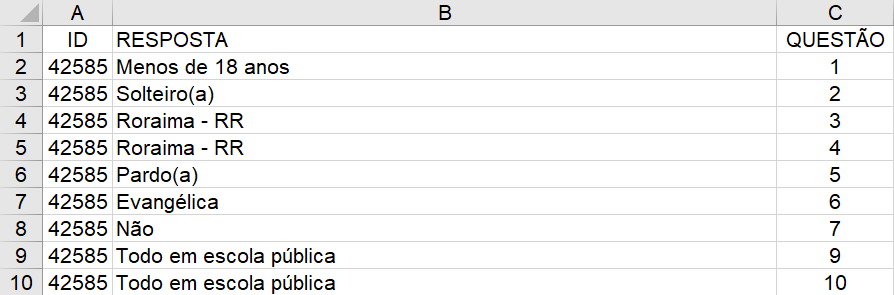
\includegraphics[scale=0.65]{Figuras/Formato_errado.png}
	\end{center}
    \legend{Fonte: Próprio autor.}
\end{figure}

\par
\textcolor{red}{Para poder começar com a utilização desses dados, foi necessário transformar toda a tabela para um formato apropriado a fim de que os aplicativos do software WEKA os suporte. De início foi feito colunas para cada número do questionário através das funções de filtro e concatenação fornecida pelo Excel, e as linhas abaixo delas seriam as respostas de cada candidato para aquela coluna especifica, como demonstrado na Figura 20. A coluna de ID foi removida já que não era necessário para a mineração, entretanto, ela foi necessária na geração de uma coluna nova rotulada de Aprovado que foi obtida através de duas tabelas contendo informações dos candidatos geral e dos candidatos aprovados.}

\par
\begin{figure}[!htp]
	\begin{center}
    \caption{\label{fig:waveform_fig} Tabela depois de formatada.}
	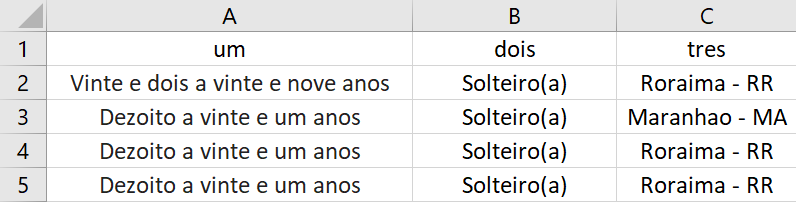
\includegraphics[scale=0.65]{Figuras/Formato_certo.png}
	\end{center}
    \legend{Fonte: Próprio autor.}
\end{figure}

\par
\textcolor{red}{O motivo dessa formatação demonstrado na Figura 20 é que o WEKA identifica a primeira linha como os atributos e as linhas subsequentes os dados relacionados a esses atributos. Como o software trabalha com formato de arquivo próprio denominado \textit{Atribute-Relation File Format} (arff), foi preciso salvar o arquivo que estava no formato xlsx para o formato csv (que separa colunas por ponto e vírgula), pois, o próprio WEKA converte esse tipo de arquivo para o tipo de arquivo que ele trabalha, o arff.}

\par
\textcolor{red}{Também foi necessário se fazer algumas alterações nas informações de dentro da tabela para que depois da conversão não viesse a ocorrer algum erro nos dados. Alterações essas como a remoção de acentos identificados nas informações da tabela, pois, os arquivos no WEKA se encontram no formato ASCII que não suportam caracteres acentuados, outra alteração foi a de transformar números para textos, pois, o tipo de dado em cada coluna só pode ser \textit{numeric nominal}, \textit{string} ou \textit{date}, e por fim, a última alteração foi a da remoção de virgulas encontradas nos dados, pois, para converter um arquivo csv no formato arff, o WEKA identifica as virgulas como as colunas que separam os dados.}

\par
\textcolor{red}{A última alteração que precisou ser feita foi da transformação dos ponto e vírgula para somente virgula, pois, o Excel ao transformar um arquivo em xlsx para csv, ele faz com a separação da coluna seja feita por ponto e vírgula o que acaba ocasionando erros e inconsistência nos dados quando o arquivo é convertido do csv para o arff, pois, o WEKA considera o caractere virgula como a representação das colunas que separam os dados. Após ter feito todos esses processos que foram mencionados anteriormente, a conversão do arquivo foi um sucesso, não tendo sido encontrado nenhum problema e inconsistência nos dados que possam ocasionar erro durante o processo de mineração.}


\subsection{Arquivo ARFF}

\par
\textcolor{}{}